\documentclass[12pt]{beamer}
% \usetheme{umbc4}
\usetheme{moloch}

\usepackage{amsmath,amscd}
\usepackage{fontspec}
\usepackage{unicode-math}
\usepackage{pifont}
\usepackage{xcolor}
\usepackage[dvipsnames]{xcolor}

\definecolor{midgray}{rgb}{0.65, 0.65, 0.65}

% Set the slide body to black background with white text
\setbeamercolor{background canvas}{bg=black}
\setbeamercolor{normal text}{fg=white}

% Set the title bar to black background with white text
\setbeamercolor{frametitle}{bg=black, fg=white}

% Ensure other structural elements (bullets, etc.) are visible
\setbeamercolor{structure}{fg=white}

\setmainfont{Libertinus Serif}
\setsansfont{Libertinus Sans}
\setmathfont{STIX Two Math}

\newcommand{\FrameTitle}[2]{\frametitle{#1 \hfill \small\textnormal{\textcolor{midgray}{#2}}}}
\newcommand{\snl}{\vspace*{3pt}\\}
\newcommand{\nl}{\vspace*{1em}\\}
\newcommand{\vsp}{\vspace*{1em}}
\newcommand{\vspthreept}{\vspace*{3pt}}

\definecolor{VeyLightBlue}{rgb}{0.65, 0.8, 1.0}
\definecolor{IceBlue}{rgb}{0.6, 0.9, 0.93}

\begin{document}
\title{\center{A Very Brief Introduction to \\ Quantum Computing \textit{and} \\ Quantum Threats \\}}
\author{\center{Manipal School of Information Sciences \\ Manipal \\}}
\date{\center{Friday, 24 April 2026}}
\maketitle

\begin{frame}\FrameTitle{What is Quantum Computing?}{QC-QIT}
    \textit{A quantum computer is one whose operation exploits certain very
    special transformations of its state...}\nl

    \textit{The laws of quantum mechanics allow these peculiar transformations
    to take place under very carefully controlled conditions.}\nl

    \vspace*{2em}
    {\hfill\color{VeyLightBlue}N. David Mermin}\\\vspthreept
    {\hfill\color{VeyLightBlue}Quantum Computer Science - An Introduction}\\
\end{frame}

\begin{frame}\FrameTitle{What is Quantum Computing?}{QC-QIT}
    \textit{The new paradigm demonstrates that the theory of computation
    can depend profoundly on the physics of the devices that carry it out.}\nl

    \textit{By focussing extensively on how quantum mechanics enlarges the possibilities
    for the physical manipulation of digital information, it is possible to characterize
    how the quantum theory works in an elementary and quite concrete way...}\nl

    \vspace*{2em}
    {\hfill\color{VeyLightBlue}N. David Mermin}\\\vspthreept
    {\hfill\color{VeyLightBlue}Quantum Computer Science - An Introduction}\\
\end{frame}

\begin{frame}\FrameTitle{What is Quantum Computing?}{QC-QIT}
    Quantum computers can solve a class of problems that are believed to be computationally hard
    to solve on classical computers.\nl

    Quantum computers are built to \textit{control} and \textit{harness} quantum phenomena such as
    {\color{VeyLightBlue}\textbf{superposition}} and {\color{VeyLightBlue}\textbf{entanglement}}
    enabling massive parallelism.\nl
\end{frame}

\begin{frame}\FrameTitle{Quantum Information Theory}{QC-QIT}
    $$
        \overbrace{\begin{array}{ll}
            & \text{\large{Quantum Information Theory}} = \vspace*{1em}\\
            &\text{\normalsize\color{lightgray}{${20}^{\text{th}}$\text{Century}}}
            \begin{cases}
            & \text{\large{Quantum Theory}} \quad \ \, + \vspace*{4pt}\\
            & \text{\large{Computer Science}} \quad + \vspace*{4pt}\\
            & \text{\large{Information Theory}} \vspace*{2pt}\\
            \end{cases}
        \end{array}}^{\text{\normalsize\color{orange}{$21^{\text{st}}$ \ Century Science}}}
    $$
    \vspace*{4pt}
    Quantum error correction and quantum fault tolerance are also crucial for building large-scale quantum computers.
\end{frame}

\begin{frame}\FrameTitle{Disentangling Hype from Practicality}{QC-QIT}
    Quantum Computing is \textit{not} useful for every computing task.

    \center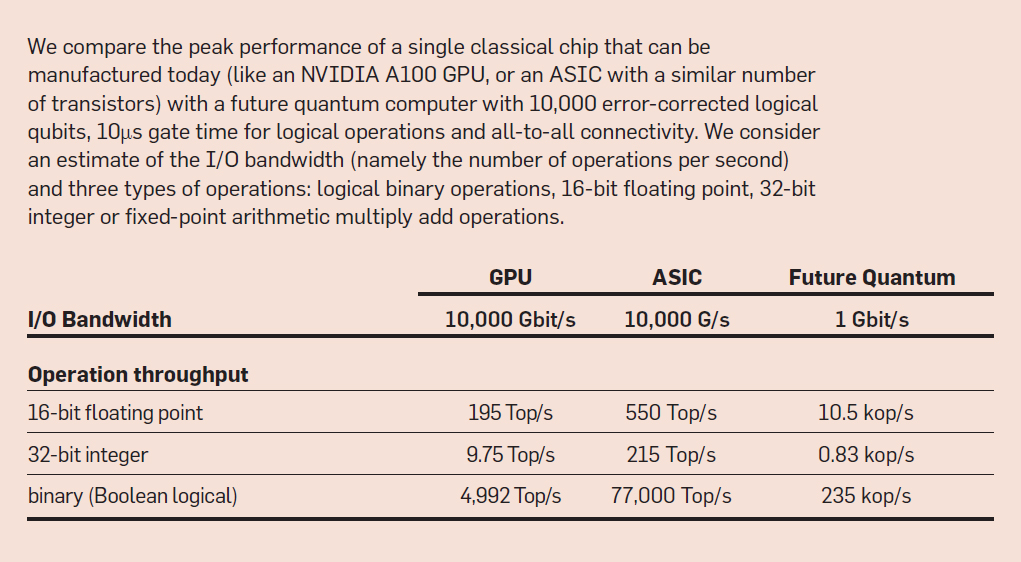
\includegraphics[width=0.8\textwidth]{images/perf-comparison.jpg}
\end{frame}

\begin{frame}\FrameTitle{Disentangling Hype from Practicality}{QC-QIT}
    Quantum Computing is \textit{not} useful for every computing task.

    \center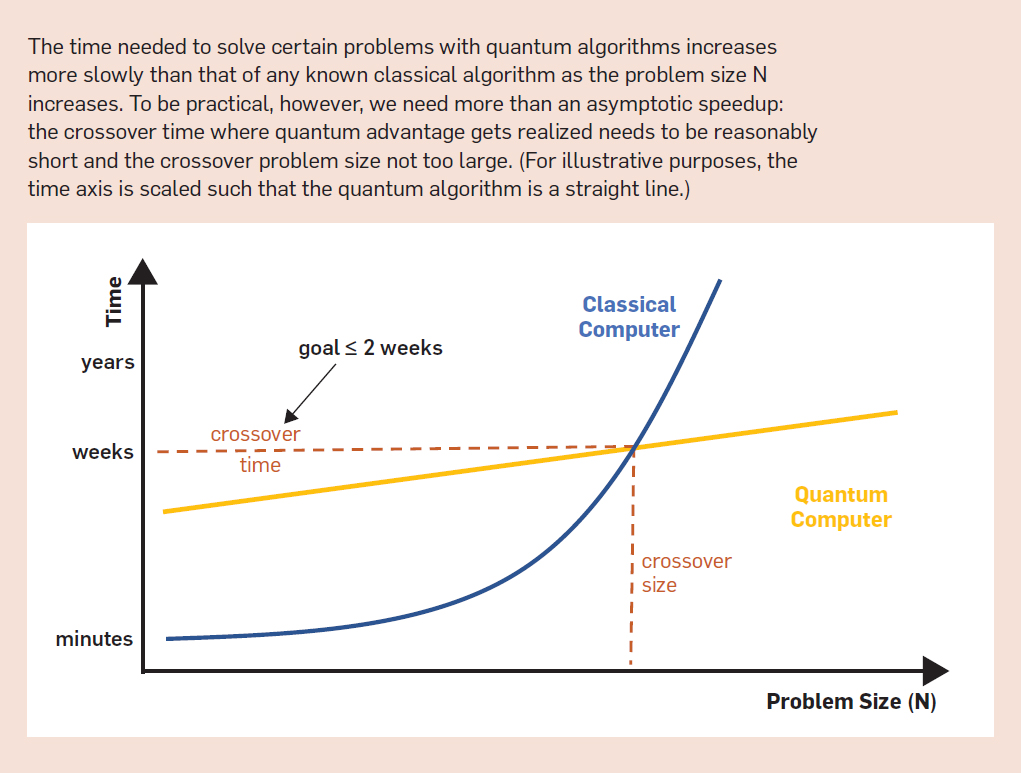
\includegraphics[width=0.8\textwidth]{images/quantum-advantage-crossover.jpg}
\end{frame}

\begin{frame}\FrameTitle{Problems Amenable to Quantum Computing}{}
    \begin{itemize}
        \item small-data big-compute tasks
        \begin{itemize}
            \item integer factoring
            \item discrete logarithm
            \item \textbf{NOT} unstructured search (Grover's algorithm)
        \end{itemize}
        \item quantum simulation (e.g., chemistry, materials science)
        \begin{itemize}
            \item input descriptions of the system being simulated are much
                smaller than the computation required to find the required properties
                of the system
        \end{itemize}
    \end{itemize}
\end{frame}


\begin{frame}\FrameTitle{Problems Amenable to Quantum Computing}{}
    \begin{itemize}
        \item Problem must have some structure that can be exploited by a quantum algorithm
        \begin{itemize}
            \item periodicity in Shor's algorithm for integer factorization
        \end{itemize}
    \end{itemize}
\end{frame}

\begin{frame}\FrameTitle{Problems Amenable to Quantum Computing}{}
    \begin{itemize}
        \item Asymptotic of the quantum algorithm must be better than the best known classical algorithm
    \end{itemize}
\end{frame}


\begin{frame}\FrameTitle{BPP}{BPP}
    A problem is in \textbf{BPP} if there is an algorithm for it that has the following properties:
    \begin{itemize}
        \item It is allowed to flip coins and make random decisions
        \item It is guaranteed to run in polynomial time
        \item On any given run of the algorithm, it has a probability of at most $\frac{1}{3}$ of
              giving the wrong answer, whether the answer is YES or NO.
    \end{itemize}
\end{frame}

\begin{frame}\FrameTitle{BPP}{BPP}
    \textbf{BPP} is the class of decision problems solvable by a probabilistic Turing machine in
    polynomial time with an error probability bounded by $\frac{1}{3}$ for all instances.\nl

    \textbf{BPP}  also contains \textbf{P}, the class of problems solvable in
    polynomial time with a deterministic machine.\nl

    Deterministic algorithm is a special case of a probabilistic algorithm.
\end{frame}


\begin{frame}\FrameTitle{Problems Amenable to Quantum Computing}{BQP}
    A problem is in NP if a solution can be verified in polynomial time by
    a deterministic Turing machine.\nl

    A problem is in \textbf{BQP} if it can be solved in polynomial time by a
    quantum Turing machine with bounded error probability.\nl
\end{frame}


\begin{frame}\FrameTitle{Problems Amenable to Quantum Computing}{BQP}
    \vspace*{4pt}
        A decision problem is a member of \textbf{BQP} if there exists a quantum algorithm
        that solves the decision problem with high probability, and is guaranteed
        to run in polynomial time. \vsp\nl
        A run of the algorithm will correctly solve the decision problem with a probability of at least $\frac{2}{3}$.
\end{frame}


\begin{frame}\FrameTitle{PQ Status of Protocols}{QC-QIT}
    Study of Post Quantum status of Widely Used Protocols\vspace*{1pt} \\
    \quad -- \url{https://arxiv.org/pdf/2603.28728v1}
\end{frame}

\begin{frame}\FrameTitle{-}{QC-QIT}
\end{frame}

\begin{frame}\FrameTitle{-}{QC-QIT}
\end{frame}

\begin{frame}\FrameTitle{-}{QC-QIT}
\end{frame}

\end{document}